\documentclass[%
 reprint,
%superscriptaddress,
%groupedaddress,
%unsortedaddress,
%runinaddress,
%frontmatterverbose, 
%preprint,
%showpacs,preprintnumbers,
%nofootinbib,
%nobibnotes,
%bibnotes,
 amsmath,amssymb,
 aps,
%pra,
%prb,
%rmp,
%prstab,
%prstper,
%floatfix,
]{revtex4-1}

\usepackage{graphicx}% Include figure files
\usepackage{dcolumn}% Align table columns on decimal point
\usepackage{bm}% bold math
%\usepackage{hyperref}% add hypertext capabilities
%\usepackage[mathlines]{lineno}% Enable numbering of text and display math
%\linenumbers\relax % Commence numbering lines

%\usepackage[showframe,%Uncomment any one of the following lines to test 
%%scale=0.7, marginratio={1:1, 2:3}, ignoreall,% default settings
%%text={7in,10in},centering,
%%margin=1.5in,
%%total={6.5in,8.75in}, top=1.2in, left=0.9in, includefoot,
%%height=10in,a5paper,hmargin={3cm,0.8in},
%]{geometry}

\usepackage{cmap} % Поиск в PDF
\usepackage[T2A]{fontenc} % Кодировка
\usepackage[utf8]{inputenc} % Кодировка исходного текста
\usepackage[english, russian]{babel} % Локализация и переносы
\frenchspacing % Более тонкая настройка пробелов 
\usepackage{multirow}
\usepackage[warn]{mathtext}
\usepackage{amssymb}
\usepackage{ dsfont }
\usepackage{ textcomp }
\usepackage{ mathrsfs }

% Переопределение англоязычного начертания каппа, фи и эпсилон, 
% а также знаков сравнения
\renewcommand{\epsilon}{\ensuremath{\varepsilon}}
\renewcommand{\phi}{\ensuremath{\varphi}} 
\renewcommand{\kappa}{\ensuremath{\varkappa}}
\renewcommand{\le}{\ensuremath{\leslant}}
\renewcommand{\leq}{\ensuremath{\leqslant}}
\renewcommand{\ge}{\ensuremath{\geslant}}
\renewcommand{\geq}{\ensuremath{\geqslant}}
\renewcommand{\emptyset}{\ensuremath{\varnothing}}

\usepackage{textcomp} 
\usepackage{indentfirst} % Красная строка
\usepackage{amsmath} % Текст в формулах
\usepackage{graphicx} % Графика
\DeclareGraphicsExtensions{.pdf,.png,.jpg}
\usepackage{pgfplots}
\pgfplotsset{compat=1.13}

%\usepackage{times}

\begin{document}

\title{Преобразование Фурье в оптике}
\thanks{4.3.4}

\author{Иван Едигарьев}
\affiliation{
 Московский Физико-Технический Институт\\
 Факультет Общей и Прикладной Физики, 526т\\
}
%\date{\today}

\begin{abstract}
В работе предлагается: А) определить размеры щели сначала по увеличенному с помощью линзы изображению, затем — по спектру на экране; Б) определить периоды сеток сначала по спектру, затем по увеличенному изображению спектра; В) исследовать изображение щели,
мультиплицированное с помощью сеток; Г) проследить влияние щелевой диафрагмы, расположенной в фурье-плоскости, на изображение сетки.

В работе используются: гелий-неоновый лазер, кассета с набором сеток разного периода, щель с микрометрическим винтом, линзы, экран, линейка.\\

\end{abstract}

\pacs{Valid PACS appear here}% PACS, the Physics and Astronomy
                             % Classification Scheme.
%\keywords{Suggested keywords}%Use showkeys class option if keyword
                              %display desired
\maketitle

%\tableofcontent

\section{\label{sec:level1}Определение ширины щели}

\begin{center}
I. Определение ширины щели с помощью линзы
\end{center}

\begin{enumerate}

    \item 
    Включим в сеть блок питания лазера. Обратим внимание на распределение интенсивности излучения лазера на экране: на его сложную структуру, обусловленную возбуждением различных типов колебаний в резонаторе лазера.
    
    \item
    Установим тубус со щелью вплотную к выходному окну лазера (см. рис. 1). Настройку системы следует вести, наблюдая за пятном света на листе бумаги.
    
    \begin{figure}[h]
    \center{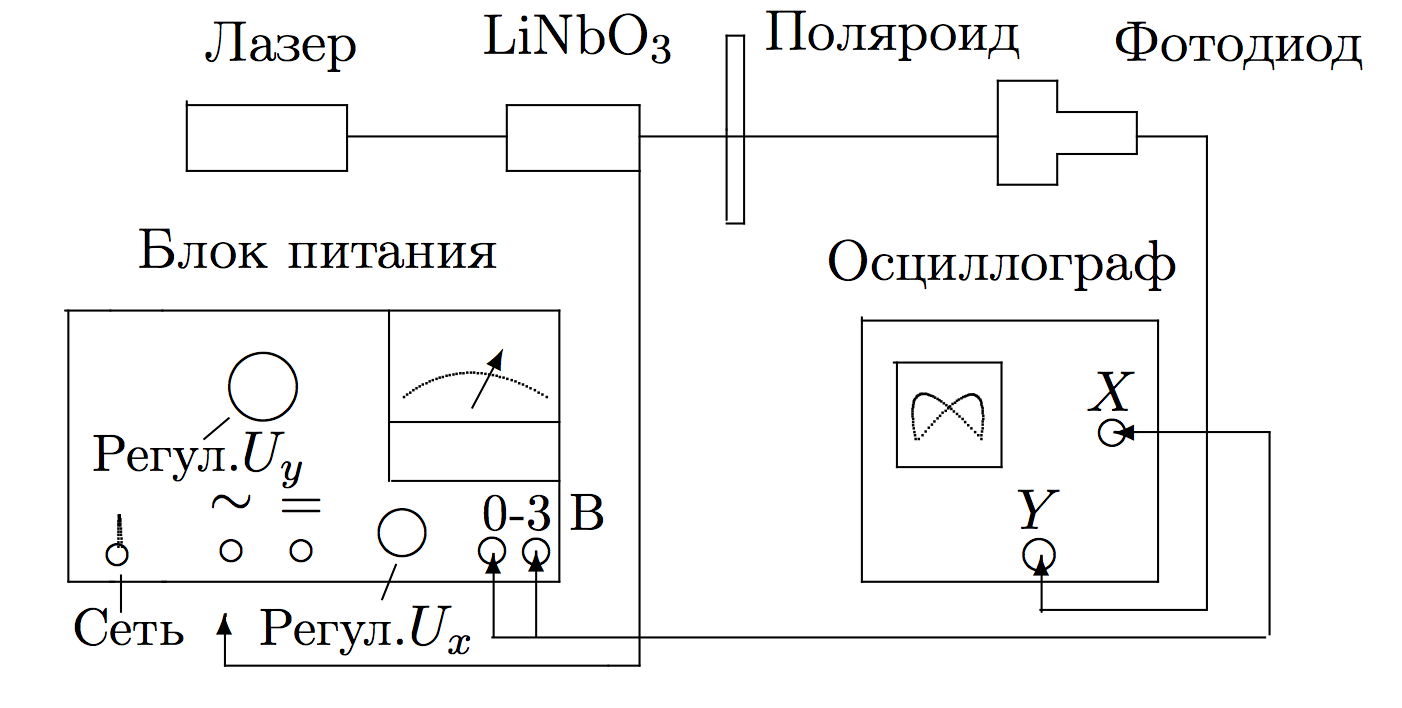
\includegraphics[scale=0.17]{pic1.png}}
    \caption{Схема для определения ширины щели с помощью линзы}
    \end{figure}
    
    \item
    С помощью короткофокусной линзы $\text{Л}_1$ ($F_1 \simeq 3-4$~см) получим на экране Э увеличенное изображение щели.
    
    \item
    Определим начало отсчёта ширины щели по её открытию, т. к. ноль может быть сбит. Цена деления винта — 10 мкм.
    $$ h_0 = 38~\text{дел}.$$
    
    \item
    Меняя ширину щели от $50$ до $500$~мкм ($5-50$ делений от нового нуля), снимем зависимость размера изображения $D_1$ от ширины щели $D$. Изменение ширины щели следует вести в сторону увеличения, чтобы исключить влияние люфта (свободного хода винта).
    
    \item 
    Измерим расстояния $a_1$ и $b_1$ для определения увеличения $\text{Г}$ системы. Погрешность этих измерений велика (особенно для малого расстояния $a_1$), поэтому, измерив дополнительно $L = a_1 + b_1$ и зная $F_1$, можно по формуле линзы рассчитать $a_1$ и $b_1$ и сравнить с измеренными. Для удалённого экрана расчёт даёт обычно $a_1 \simeq F_1$.
    \begin{gather*}
        a_1 = (43 \pm 5)~\text{mm}\\
        b_1 = (120 \pm 1)~\text{cm}\\
        L = (124 \pm 1)~\text{cm}\\
        F = 43~\text{mm}\\
        a_2 = FL/b_1 = (44 \pm 2)~\text{mm}\\
        \\
        a = (43 \pm 3)~\text{mm} \simeq F
    \end{gather*}
    
    \item
    Зная увеличение линзы и размер изображения, рассчитаем ширину входной щели $D_{\text{л}}$ («л» — с применением линзы).
        
\end{enumerate}

\begin{center}
II. Определение ширины щели по её спектру
\end{center}

\begin{enumerate}
    \item
    Получим на удалённом экране спектр щели (рис. 2). Меняя ширину щели, проследим за изменением спектра на экране и оценим интервал, для которого можно наблюдать и измерять спектр - от 40 до (130-140) дел.
    
    \begin{figure}[h]
    \center{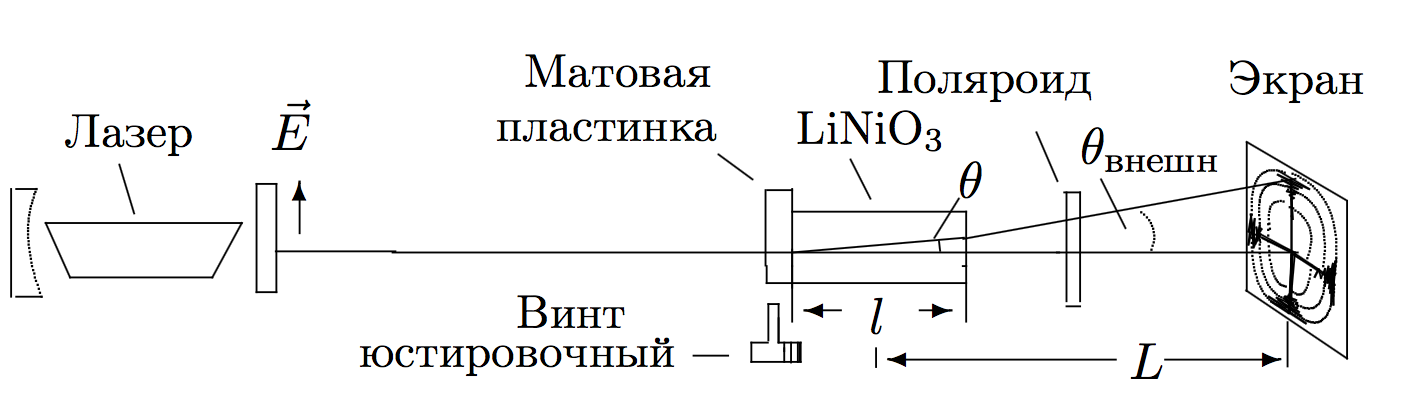
\includegraphics[scale=0.17]{pic2.png}}
    \caption{Схема для определения ширины щели по спектру}
    \end{figure}
   
    \item
    Измерим ширину спектра для самой маленькой щели. Для большей точности следует измерять расстояние $X$ между удалёнными от центра минимумами, расположенными симметрично относительно центра картины, и отмечать порядок минимума $m$ (например, 1-й, 2-й, 3-й, ..., начиная от центра).
    
    Проведём серию измерений $X(m)$, меняя ширину щели в тех же пределах, что и в п. 5.
    
    Измерим расстояние $L$ от щели до экрана.
    $$ L = (124 \pm 1)~\text{cm}$$
    
    \item
    По результатам измерений спектра рассчитаем ширину щели $D_c$ («с» — по спектру), используя соотношения
    $$ \Delta X = \frac{X}{2m} = \frac{\lambda}{D_c}L$$
    
    Длина волны Hg лазера $\lambda = 5461 \text{\AA}$.
    
    Построим на одном листе графики $D_{\text{л}} = f(D)$ и $D_c = f(D).$
    
    \begin{figure}[h]
    \center{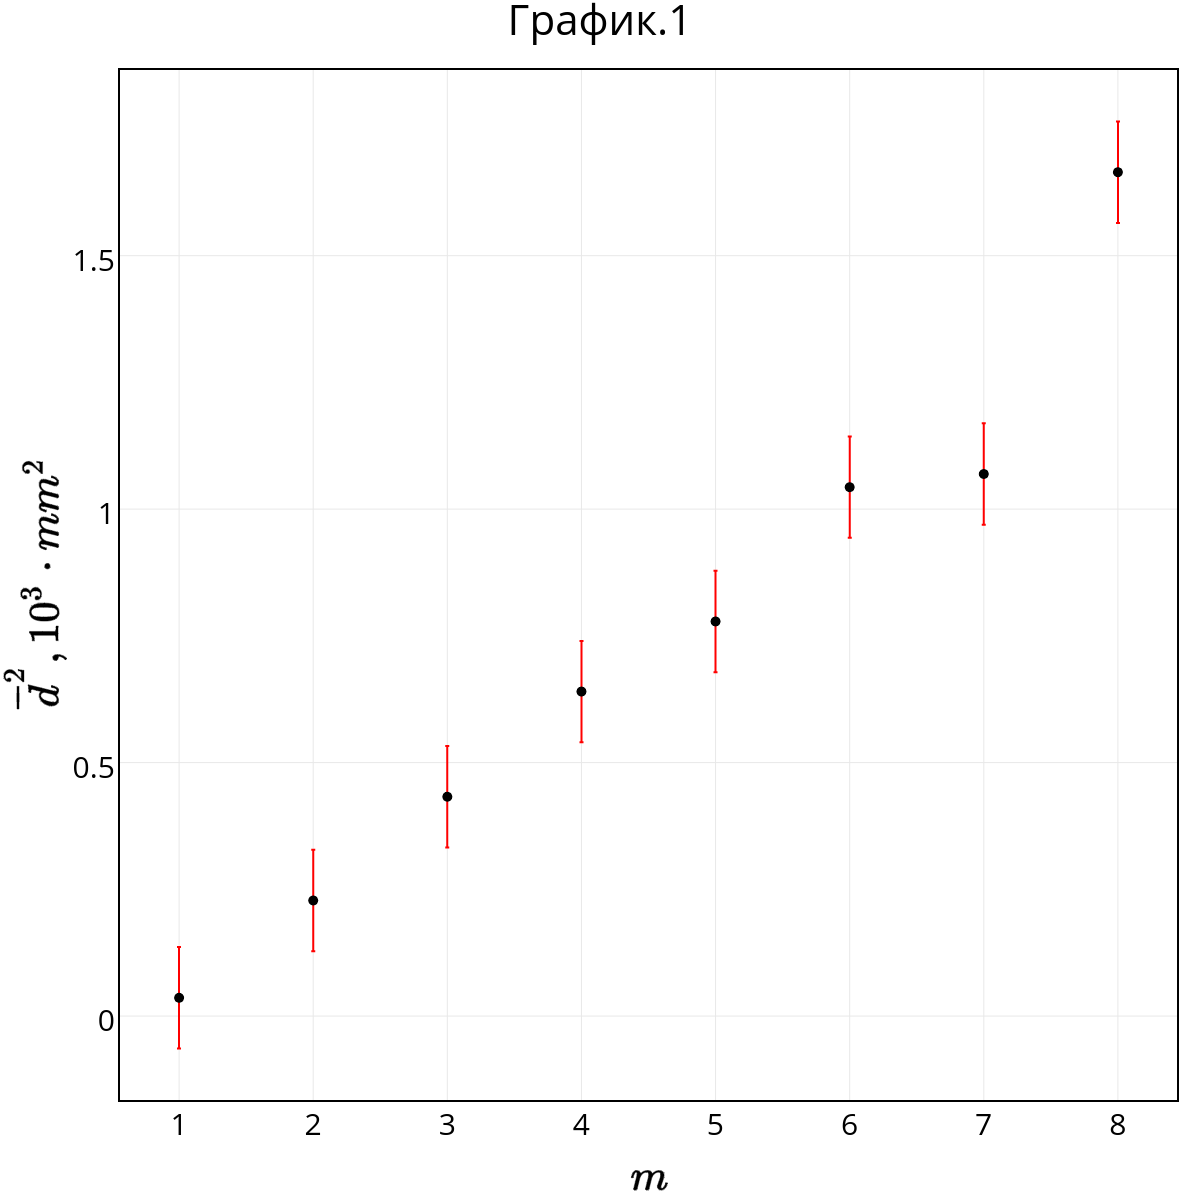
\includegraphics[scale=0.17]{my_plot1.png}}
    \end{figure}
    
\end{enumerate}

\section{\label{sec:level1}Определение периода решёток}

\begin{center}
I. Определение периода по спектру на удалённом экране
\end{center}

\begin{enumerate}
    \item
    Поставим кассету с двумерными решётками (сетками) вплотную к выходному окну лазера. В окошке под отверстием с сеткой виден \textnumero~ сетки. Вращением наружного кольца кассеты можно менять сетки.
    
    \begin{figure}[h]
    \center{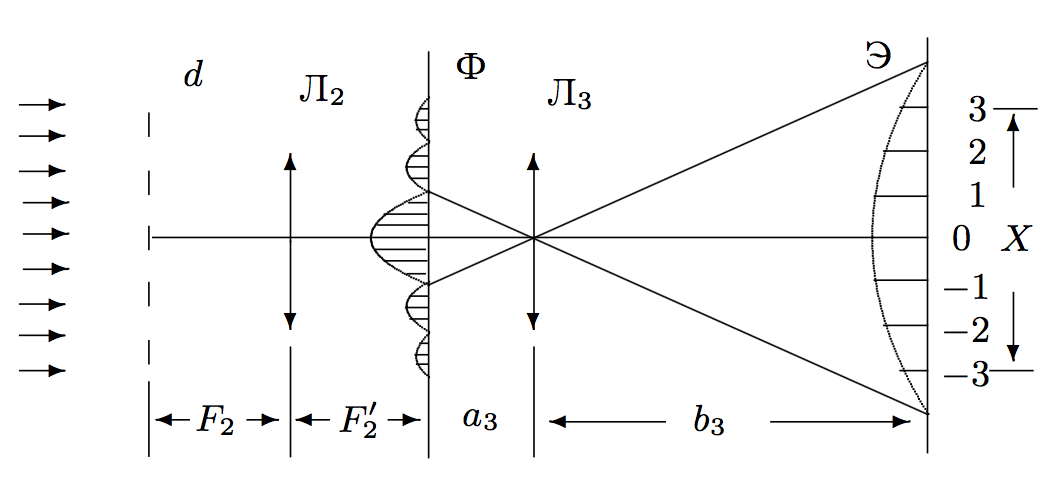
\includegraphics[scale=0.17]{pic3.png}}
    \caption{Схема определения периода решётки по увеличенному изображению спектра}
    \end{figure}
    
    \item
    Для каждой сетки измерим расстояние $X$ между $m$-ми максимумами и отметим $m$ — порядок максимума.
    
    Измерим расстояние $L$ от кассеты до экрана.
    $$ L = (120 \pm 2)~\text{cm}$$
    
    \item 
    Рассчитаем расстояния $\Delta X$ между соседними максимумами и определим период каждой решётки $d_c = f(\text{\textnumero})$, используя соотношения
    $$ \Delta X = \frac{X}{2m} = \frac{\lambda}{d_c}F$$
    Для крупных решёток спектры промерить не удаётся — они слишком узки. Их можно увеличить с помощью системы линз.
\end{enumerate}

\begin{center}
I. Определение периода решёток по увеличенному изображению спектра
\end{center}

\begin{enumerate}
    \item
    Линзу $\text{Л}_2$ с максимальным фокусом ($F_2 \simeq 10$~см) поставим на расстоянии $\simeq F_2$ от кассеты. В плоскости Ф линза $\text{Л}_2$ даёт фурье-образ сетки — её спектр, а короткофокусная линза $\text{Л}_3$~($F_3 \simeq 2,5$~см) cоздаёт на экране увеличенное изображение этого спектра.
    
    Так как экран достаточно удалён ($b_3 \gg a_3$), то практически $a_3 = F_3$, и расстояние между линзами $\simeq F_2 + F_3.$
    
    \item 
    Измерим $X$ и $m$ для всех сеток, где это возможно.
    
    \item
    Зная увеличение линзы $\text{Л}_3$ ($\text{Г}_3 = b_3/a_3$), можно рассчитать расстояние между максимумами $\Delta x$ в плоскости Ф, а затем период сетки $d_{\text{л}}$:
    $$\Delta x = \frac{\Delta X}{\text{Г}_3} = \frac{\lambda}{d_{\text{л}}}F_2.$$   
    
\end{enumerate}

\section{\label{sec:level1}Мультиплицирование}

\begin{enumerate}
    \item
    Снова поставим тубус со щелью к окну лазера (рис. 4) и найдём на экране резкое изображение щели с помощью линзы $\text{Л}_2$ ($F_2 \simeq 10$ см).
    
    В фокальной плоскости Ф линзы $\text{Л}_2$ поставим кассету с сетками, которые будут «рассекать» фурье-образ щели — осуществлять пространственную фильтрацию.
    
    \begin{figure}[h]
    \center{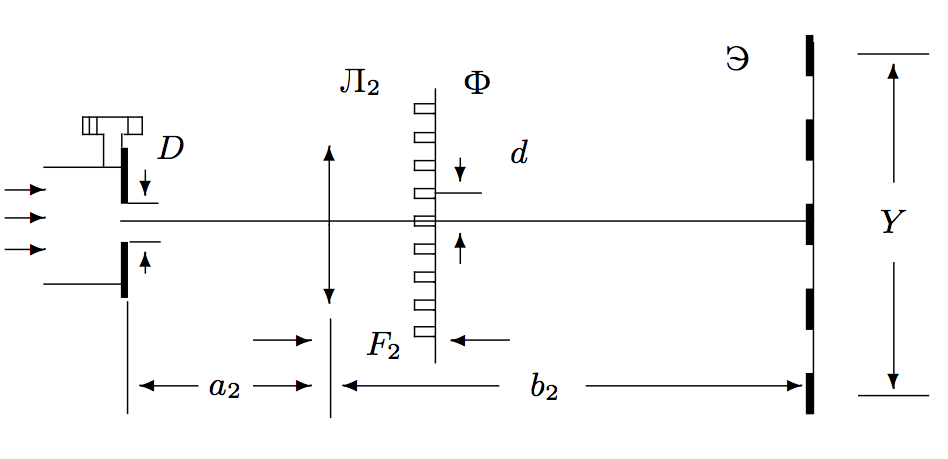
\includegraphics[scale=0.17]{pic4.png}}
    \caption{Схема для наблюдения мультиплицирования}
    \end{figure}
    
    \item
    Подберём такую ширину входной щели $D$, чтобы на экране можно было наблюдать мультиплицированное изображение для всех сеток. Чем уже щель, тем шире её фурье-образ и тем легче рассечь его сетками.
    
    \item
    Снимем зависимость $Y$ (расстояние между удалёнными изображениями щели) и $K$ (число промежутков между изображениями) от \textnumero~(номер сетки) для фиксированной ширины входной щели.
    
    Запишим величины $D$ и $F_2$. Измерим расстояния $a_2$ и $b_2$ для расчёта увеличения $\text{Г}_2$.
    
    \item
    Рассчитаем периоды $\Delta y$ «фиктивных» решёток, которые дали бы такую же периодичность на экране: $\Delta y = \Delta Y / \text{Г}_2$, где $\Delta Y = Y/K$.
    
    Построим график $\Delta y = f(1/d_c)$, где $d_c$ — периоды решёток, определённые по спектру. Зависимость должна быть линейной, поскольку
    $$\frac{\lambda}{\Delta y} F_2 = d_c$$
    \begin{figure}[h]
    \center{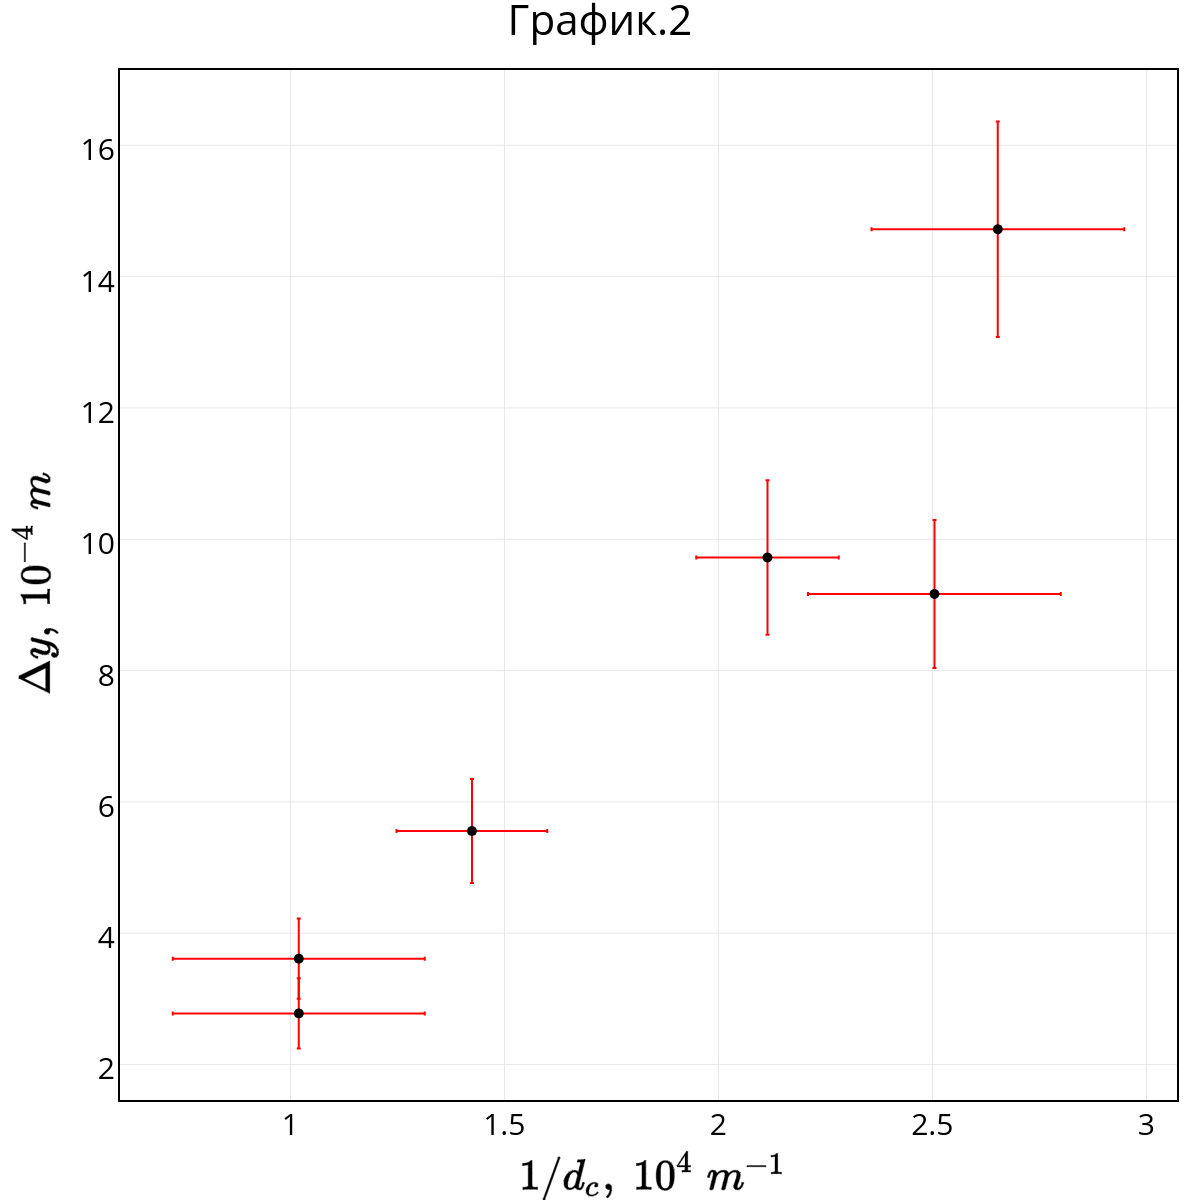
\includegraphics[scale=0.17]{my_plot2.png}}
    \end{figure}
    
    \item
    Зная размер щели $D$, построим в масштабе первичное изображение (спектр щели) и отложим на нём величины $d(\text{\textnumero})$ — периоды самой плотной и самой редкой из использованных решёток.
    
\end{enumerate}

\section{\label{sec:level1}Влияние щелевой диафрагмы на изображение сетки}

    Поставим на место щели (рис. 4) кассету с сетками и сфокусируем на экран изображение сетки. Убедимся, что изображение остаётся резким при смене сеток.

    Поставим в плоскости Ф вертикальную щель и проследим за изменением изображения на экране при сужении щели. Проделаем то же для щели, ориентированной горизонтально и под углом 45\textdegree~к вертикали.

\end{document}

